\documentclass[10pt,journal,compsoc,onecolumn]{IEEEtran}

% ---- packages ----
\usepackage[T1]{fontenc}
\usepackage[utf8]{inputenc}
\usepackage{graphicx}
\usepackage{booktabs}
\usepackage{amsmath}
\usepackage{amssymb}
\usepackage{xcolor}
\usepackage{tikz}
\usetikzlibrary{positioning,arrows.meta,calc,fit,backgrounds}
\usepackage{caption}
\usepackage{url}
\usepackage[colorlinks=true,linkcolor=blue,citecolor=blue,urlcolor=blue]{hyperref}

% IEEEtran labels the keywords block "Index Terms" by default.
\renewcommand{\IEEEkeywordsname}{Key words:}

\begin{document}

\title{FORUM-TB: An Interpretable Machine Learning Framework for Multi-Drug Resistance Prediction in \textit{Mycobacterium tuberculosis} from Whole-Genome Sequencing}

% -------------------------------------------------------------------
% AUTHOR BLOCK -- PLACEHOLDERS: fill in exact institutional affiliations
% and contact emails before submission.
% -------------------------------------------------------------------
\author{Nanzhen~(Aspen)~Qiao and Noah~LeGall%
\IEEEcompsocitemizethanks{%
\IEEEcompsocthanksitem N. Qiao is with [INSERT AFFILIATION -- INSTITUTION, DEPARTMENT], Kingston, ON, Canada.
\IEEEcompsocthanksitem N. LeGall is with [INSERT AFFILIATION -- INSTITUTION, DEPARTMENT], San Diego, CA, USA. E-mail: [INSERT EMAIL] (Corresponding author).}}

\IEEEtitleabstractindextext{%
\begin{abstract}
Drug-resistant tuberculosis remains a major global health threat, yet the diagnostics in widest use are either too slow (culture-based drug susceptibility testing, 3--16 weeks) or too narrow (GeneXpert, rifampicin only), while rule-based whole-genome sequencing catalogues provide limited quantitative interpretability at the level of an individual isolate. Here we present FORUM-TB, an open and reproducible framework that converts public \textit{Mycobacterium tuberculosis} sequencing data into interpretable, multi-drug resistance predictions. We assembled a machine-learning-ready feature matrix from 9{,}798 publicly available isolates, encoding 2{,}693 nucleotide positions across nine genes associated with resistance to the four first-line drugs (rifampicin, isoniazid, ethambutol, and pyrazinamide), and benchmarked seven classifiers per drug alongside a multi-label formulation that predicts all four drugs jointly. Random Forest achieved the highest cross-validated AUC-ROC for every drug (rifampicin 0.969, isoniazid 0.946, ethambutol 0.900, pyrazinamide 0.883), consistently outperforming gradient-boosted and linear alternatives. Applying SHAP (SHapley Additive exPlanations) to the resulting models recovered the canonical resistance-determining mutations \textit{rpoB} S450L, \textit{katG} S315T, and \textit{embB} M306I/V as top-ranked features without these associations being supplied as prior knowledge, and a cross-drug attribution analysis quantified how the importance of shared features shifts under co-resistance. The multi-label extension reached a macro AUC-ROC of 0.919 but a markedly lower four-way exact-match accuracy of 0.591, indicating that joint multi-drug profiling is substantially harder than per-drug discrimination. These results show that an interpretable, per-drug ensemble built entirely from public data and open-source tooling recovers established resistance biology while surfacing quantitative co-resistance signal that static catalogues do not expose. The dataset, code, trained models, and an interactive dashboard are released openly to support reproducible benchmarking of interpretable resistance prediction.

\end{abstract}

\begin{IEEEkeywords}
Tuberculosis, antimicrobial resistance, whole-genome sequencing, machine learning, explainable AI, SHAP.
\end{IEEEkeywords}}

\maketitle
\IEEEdisplaynontitleabstractindextext
\IEEEpeerreviewmaketitle

\section*{Introduction}

Tuberculosis (TB) remains one of the leading causes of death from a single infectious agent worldwide, and drug-resistant TB (DR-TB) is a persistent obstacle to global control efforts \cite{who2025globaltb}. Timely, drug-specific resistance information is essential to select an effective treatment regimen, yet the diagnostic tools in widest use fall short in one of two ways. Culture-based phenotypic drug susceptibility testing (DST), the historical reference standard, requires 3 to 16 weeks to return a result because \emph{Mycobacterium tuberculosis} is slow-growing. Rapid molecular assays such as GeneXpert MTB/RIF shorten this to hours but report resistance to rifampicin only, leaving isoniazid, ethambutol, and pyrazinamide resistance undetermined \cite{helb2010genexpert}.

Whole-genome sequencing (WGS) offers a path to same-day, multi-drug resistance prediction directly from sequence data, and several large-scale efforts have demonstrated that WGS-derived genotype can predict phenotypic resistance with high concordance across many drugs simultaneously \cite{walker2015whole,cryptic2022compendium}. Standardized resistance catalogues, most notably the World Health Organization's catalogue of mutations, formalize this genotype-to-phenotype mapping as a curated, rule-based lookup \cite{who2023catalogue}. Rule-based catalogues are transparent in the sense that each listed mutation has an explicit, documented resistance association, but they do not produce a quantitative, per-isolate explanation of a prediction, cannot easily represent the combined effect of multiple co-occurring variants, and require periodic manual re-curation as new mutations are characterized.

Machine learning (ML) classifiers trained directly on genomic features can, in principle, capture combinations of variants and continuous-valued statistical structure that a fixed mutation list does not, but historically ML models have been criticized for functioning as opaque predictors that a clinician or microbiologist cannot audit. SHAP (SHapley Additive exPlanations) addresses this gap by attributing each individual prediction to a signed, per-feature contribution that sums to the model's output, drawing on a game-theoretic foundation for feature attribution \cite{lundberg2017unified}. Applying SHAP to a tree-based ensemble trained on genomic features makes it possible to ask, for a specific isolate, which genomic positions drove a specific resistance prediction, and to check those positions against known resistance biology.

In this work we present FORUM-TB, an open, reproducible pipeline (Fig.~\ref{fig:pipeline}) that (i) constructs an ML-ready, nucleotide-encoded SNP feature matrix for \emph{M. tuberculosis} from public WGS data restricted to nine genes associated with resistance to the four first-line ("RIPE") drugs -- rifampicin, isoniazid, ethambutol, and pyrazinamide; (ii) benchmarks seven standard classifiers per drug, and extends the best-performing model family to a multi-label formulation that predicts all four drugs jointly; (iii) applies SHAP to interpret per-drug and per-isolate predictions, including a cross-drug attribution analysis that quantifies how a shared feature's importance shifts under co-resistance; and (iv) releases the dataset, trained models, and an interactive dashboard publicly to support reproducible benchmarking of interpretable AMR prediction models. Our central aim is not to outperform existing WGS-to-resistance tools on raw accuracy, but to demonstrate that a fully interpretable, multi-drug pipeline built from public data and open-source tooling recovers established resistance biology while surfacing quantitative co-resistance signal that a static catalogue cannot.

% Overview schematic of the FORUM-TB framework (modelled on the layout of
% Fig. 1 in the reference preprint: staged, left-to-right framework overview).
%
% Layout: nodes sit on a fixed (column, row) grid with a uniform box height, so
% that rows align across all five stages and every column ends at the same
% baseline. Do not switch back to relative "below=of" chaining -- boxes grow
% with their text and the rows drift out of alignment.
\begin{figure*}[t]
\centering
\resizebox{\textwidth}{!}{%
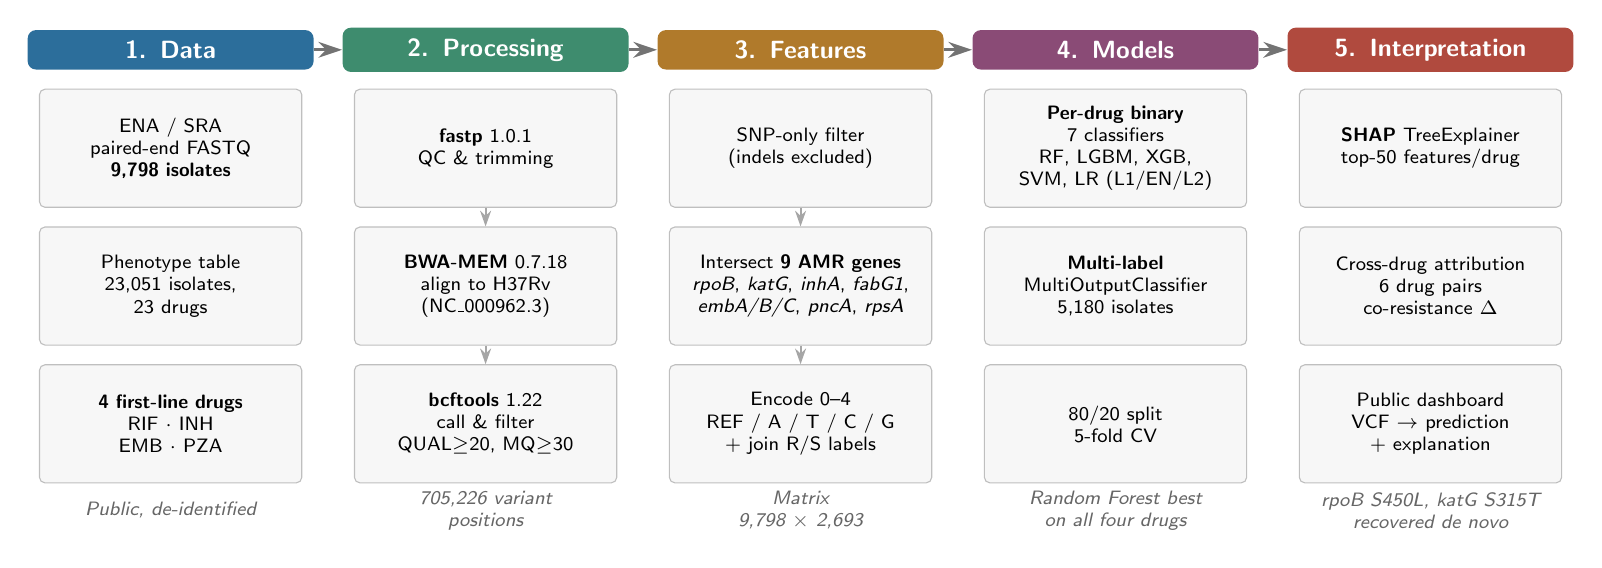
\begin{tikzpicture}[
  font=\sffamily\small,
  hdr/.style={
    rounded corners=3pt, draw=none, fill=#1,
    text width=3.35cm, align=center, inner sep=4pt,
    font=\sffamily\bfseries\small, text=white},
  item/.style={
    rounded corners=2pt, draw=black!25, fill=black!3,
    text width=3.05cm, align=center, inner sep=4pt,
    font=\sffamily\scriptsize,
    minimum height=1.5cm},          % sized for the tallest box (4 text lines)
  note/.style={font=\sffamily\scriptsize\itshape, text=black!60, align=center,
    text width=3.3cm},
  flow/.style={-{Stealth[length=3mm,width=2mm]}, line width=1.1pt, draw=black!55},
  sub/.style={-{Stealth[length=2mm,width=1.4mm]}, line width=0.7pt, draw=black!35}
]

% ---- palette ----
\definecolor{cData}{HTML}{2C6E9B}
\definecolor{cProc}{HTML}{3E8C6E}
\definecolor{cFeat}{HTML}{B07A2B}
\definecolor{cModel}{HTML}{8A4B76}
\definecolor{cInt}{HTML}{B04A3E}

% ---- grid ----------------------------------------------------------------
% Column centres: 0, 4, 8, 12, 16.  Row centres: headers 0, then -1.25 /
% -3.00 / -4.75 (1.75 pitch, 1.5 box height => 0.25 gap), notes at -5.85.
\def\rowA{-1.25}
\def\rowB{-3.00}
\def\rowC{-4.75}
\def\rowN{-5.85}

% ================= column headers =================
\node[hdr=cData]  (h1) at (0,0)    {1. Data};
\node[hdr=cProc]  (h2) at (4,0)    {2. Processing};
\node[hdr=cFeat]  (h3) at (8,0)    {3. Features};
\node[hdr=cModel] (h4) at (12,0)   {4. Models};
\node[hdr=cInt]   (h5) at (16,0)   {5. Interpretation};

% ================= column 1: data =================
\node[item] (d1) at (0,\rowA) {ENA / SRA\\ paired-end FASTQ\\ \textbf{9{,}798 isolates}};
\node[item] (d2) at (0,\rowB) {Phenotype table\\ 23{,}051 isolates,\\ 23 drugs};
\node[item] (d3) at (0,\rowC) {\textbf{4 first-line drugs}\\ RIF $\cdot$ INH\\ EMB $\cdot$ PZA};
\node[note] (n1) at (0,\rowN) {Public, de-identified};

% ================= column 2: processing =================
\node[item] (p1) at (4,\rowA) {\textbf{fastp} 1.0.1\\ QC \& trimming};
\node[item] (p2) at (4,\rowB) {\textbf{BWA-MEM} 0.7.18\\ align to H37Rv\\ (NC\_000962.3)};
\node[item] (p3) at (4,\rowC) {\textbf{bcftools} 1.22\\ call \& filter\\ QUAL$\geq$20, MQ$\geq$30};
\node[note] (n2) at (4,\rowN) {705{,}226 variant\\ positions};

% ================= column 3: features =================
\node[item] (f1) at (8,\rowA) {SNP-only filter\\ (indels excluded)};
\node[item] (f2) at (8,\rowB) {Intersect \textbf{9 AMR genes}\\ \textit{rpoB}, \textit{katG}, \textit{inhA}, \textit{fabG1},\\ \textit{embA/B/C}, \textit{pncA}, \textit{rpsA}};
\node[item] (f3) at (8,\rowC) {Encode 0--4\\ REF / A / T / C / G\\ + join R/S labels};
\node[note] (n3) at (8,\rowN) {Matrix\\ 9{,}798 $\times$ 2{,}693};

% ================= column 4: models =================
\node[item] (m1) at (12,\rowA) {\textbf{Per-drug binary}\\ 7 classifiers\\ RF, LGBM, XGB,\\ SVM, LR (L1/EN/L2)};
\node[item] (m2) at (12,\rowB) {\textbf{Multi-label}\\ MultiOutputClassifier\\ 5{,}180 isolates};
\node[item] (m3) at (12,\rowC) {80/20 split\\ 5-fold CV};
\node[note] (n4) at (12,\rowN) {Random Forest best\\ on all four drugs};

% ================= column 5: interpretation =================
\node[item] (i1) at (16,\rowA) {\textbf{SHAP} TreeExplainer\\ top-50 features/drug};
\node[item] (i2) at (16,\rowB) {Cross-drug attribution\\ 6 drug pairs\\ co-resistance $\Delta$};
\node[item] (i3) at (16,\rowC) {Public dashboard\\ VCF $\rightarrow$ prediction\\ + explanation};
\node[note] (n5) at (16,\rowN) {\textit{rpoB} S450L, \textit{katG} S315T\\ recovered \textit{de novo}};

% ================= inter-stage flow arrows (stage-level, not node-level) ====
\draw[flow] (h1.east) -- (h2.west);
\draw[flow] (h2.east) -- (h3.west);
\draw[flow] (h3.east) -- (h4.west);
\draw[flow] (h4.east) -- (h5.west);

% ================= intra-column flow arrows =================
\foreach \a/\b in {p1/p2, p2/p3, f1/f2, f2/f3} {\draw[sub] (\a) -- (\b);}

\end{tikzpicture}}
\caption{\textbf{Overview of the FORUM-TB framework.} Publicly available \textit{M. tuberculosis} whole-genome sequencing runs and their phenotypic drug-susceptibility labels are processed through a standardized read-to-variant pipeline, reduced to a nucleotide-encoded SNP feature matrix restricted to nine antimicrobial-resistance genes, and used to train per-drug and multi-label classifiers for the four first-line drugs. The best-performing models are then interpreted with SHAP, both per drug and across drug pairs, and deployed in a public dashboard that returns a resistance profile and its per-feature explanation for a user-supplied VCF.}
\label{fig:pipeline}
\end{figure*}



\section*{Results}

\subsection*{Dataset and evaluation}

We assembled a nucleotide-encoded SNP feature matrix from 9{,}798 publicly available \emph{M. tuberculosis} isolates, comprising 2{,}693 positions across nine genes associated with resistance to the four first-line drugs (Methods; Fig.~\ref{fig:pipeline}). Phenotypic label availability differs by drug, reflecting which isolates were tested against which agent in the source studies: 9{,}630 isolates for rifampicin, 9{,}580 for isoniazid, 8{,}196 for ethambutol, and 5{,}749 for pyrazinamide (Table~\ref{tab:dataset}). Class balance also varies substantially, from near-parity for ethambutol (49.8\% resistant) and pyrazinamide (45.4\% resistant) to strongly resistant-skewed for isoniazid (86.0\% resistant). All models were evaluated on an 80/20 stratified train/test split with 5-fold stratified cross-validation on the training partition, reporting accuracy and AUC-ROC; the multi-label formulation was additionally assessed by Hamming loss and subset (exact-match) accuracy.

\begin{table}[h]
\centering
\caption{Dataset summary. Isolates and per-drug phenotype label counts after quality-control filtering (3 outliers removed: ERR1034652, ERR1035353, ERR1213920).}
\label{tab:dataset}
\begin{tabular}{lrrr}
\toprule
Drug & Labelled isolates & Resistant, n (\%) & Susceptible, n (\%) \\
\midrule
Rifampicin   & 9{,}630 & 7{,}144 (74.2\%) & 2{,}486 (25.8\%) \\
Isoniazid    & 9{,}580 & 8{,}238 (86.0\%) & 1{,}342 (14.0\%) \\
Ethambutol   & 8{,}196 & 4{,}082 (49.8\%) & 4{,}114 (50.2\%) \\
Pyrazinamide & 5{,}749 & 2{,}610 (45.4\%) & 3{,}139 (54.6\%) \\
\bottomrule
\end{tabular}

\vspace{4pt}
\footnotesize
Total isolates in the final feature matrix: 9{,}798. Feature count: 2{,}693 nucleotide-encoded SNP positions across nine AMR genes (\emph{rpoB}; \emph{katG}, \emph{inhA}, \emph{fabG1}; \emph{embB}, \emph{embA}, \emph{embC}; \emph{pncA}, \emph{rpsA}). The underlying phenotype table covers 23{,}051 isolates across 23 drugs; only the four first-line drugs above are modelled here.
\end{table}


\subsection*{Per-drug classifier performance}

Across all four first-line drugs, Random Forest achieved the highest cross-validated AUC-ROC among the seven benchmarked classifiers (Table~\ref{tab:modelcomparison}), and its final per-drug models achieved test-set AUC-ROC of 0.976 (rifampicin), 0.947 (isoniazid), 0.894 (ethambutol), and 0.886 (pyrazinamide), with corresponding 5-fold CV AUC-ROC of 0.969, 0.946, 0.900, and 0.883 (Table~\ref{tab:perdrug}). Gradient-boosted alternatives (LightGBM, XGBoost) tracked Random Forest closely on rifampicin and isoniazid but fell further behind on ethambutol and pyrazinamide; the linear SVM trained via SGD was the weakest model on every drug, most markedly on ethambutol (CV AUC-ROC 0.780 vs. 0.900 for Random Forest). Performance ordering across drugs (rifampicin~$>$~isoniazid~$>$~ethambutol~$\approx$~pyrazinamide) was consistent between the per-drug models (Table~\ref{tab:perdrug}) and the independent multi-model benchmarking run (Table~\ref{tab:modelcomparison}).

\begin{table}[h]
\centering
\caption{Per-drug Random Forest classifier performance (final v2 models; 80/20 stratified train/test split, 300 trees, \texttt{class\_weight="balanced"}). CV columns report 5-fold stratified cross-validation, mean $\pm$ SD.}
\label{tab:perdrug}
\begin{tabular}{lrrrr}
\toprule
Drug & Test Acc. & Test AUC-ROC & CV Acc. & CV AUC-ROC \\
\midrule
Rifampicin   & 0.9496 & 0.9759 & 0.9366 $\pm$ 0.0040 & 0.9688 $\pm$ 0.0039 \\
Isoniazid    & 0.9045 & 0.9473 & 0.9056 $\pm$ 0.0037 & 0.9462 $\pm$ 0.0074 \\
Ethambutol   & 0.8091 & 0.8936 & 0.8208 $\pm$ 0.0048 & 0.8996 $\pm$ 0.0066 \\
Pyrazinamide & 0.8200 & 0.8862 & 0.8116 $\pm$ 0.0133 & 0.8831 $\pm$ 0.0075 \\
\bottomrule
\end{tabular}

\vspace{4pt}
\footnotesize
Per-class precision/recall/F1 (test split): Rifampicin -- Susceptible 0.86/0.95/0.91, Resistant 0.98/0.95/0.97 ($n=1{,}926$); Isoniazid -- Susceptible 0.61/0.91/0.73, Resistant 0.98/0.90/0.94 ($n=1{,}916$); Ethambutol -- Susceptible 0.78/0.86/0.82, Resistant 0.84/0.76/0.80 ($n=1{,}640$); Pyrazinamide -- Susceptible 0.80/0.89/0.84, Resistant 0.85/0.74/0.79 ($n=1{,}150$).
\end{table}

\begin{table}[h]
\centering
\caption{Seven-model benchmark, 5-fold stratified cross-validation AUC-ROC per drug (independent benchmarking run from the per-drug models in Table~\ref{tab:perdrug}; minor numeric differences between the two tables reflect independent train/test splits, not a discrepancy). Bold marks the best CV AUC-ROC per drug.}
\label{tab:modelcomparison}
\small
\begin{tabular}{lrrrr}
\toprule
Model & Rifampicin & Isoniazid & Ethambutol & Pyrazinamide \\
\midrule
Random Forest        & \textbf{0.9690} & \textbf{0.9464} & \textbf{0.8997} & \textbf{0.8831} \\
LightGBM              & 0.9675 & 0.9391 & 0.8938 & 0.8699 \\
XGBoost                & 0.9643 & 0.9364 & 0.8840 & 0.8595 \\
LR L1 (Lasso)          & 0.9607 & 0.9433 & 0.8696 & 0.8660 \\
LR ElasticNet          & 0.9602 & 0.9428 & 0.8651 & 0.8614 \\
LR L2 (Ridge)          & 0.9568 & 0.9382 & 0.8569 & 0.8488 \\
Linear SVM (SGD)       & 0.9155 & 0.8782 & 0.7796 & 0.7912 \\
\bottomrule
\end{tabular}

\vspace{4pt}
\footnotesize
Same 80/20 train/test split and 5-fold stratified CV protocol as Table~\ref{tab:perdrug}, run independently per model family.
\end{table}


\subsection*{SHAP-based interpretability}

SHAP summary plots for the four per-drug Random Forest models (Figure~\ref{fig:shap_summary}) show that the top-ranked feature for rifampicin and isoniazid corresponds to a single dominant genomic position each, consistent with the well-characterized resistance mutations \emph{rpoB} S450L and \emph{katG} S315T, respectively. For ethambutol, attribution is more distributed across multiple \emph{embB} positions, consistent with the polygenic and comparatively lower discriminative performance observed in Table~\ref{tab:perdrug}. These associations were not supplied to the model as prior knowledge; they emerge purely from feature importance on the encoded SNP matrix, providing a form of internal validation that the classifiers are learning biologically plausible signal rather than confounded artefacts.

\begin{figure}[h]
\centering
\begin{minipage}{0.48\textwidth}
\centering
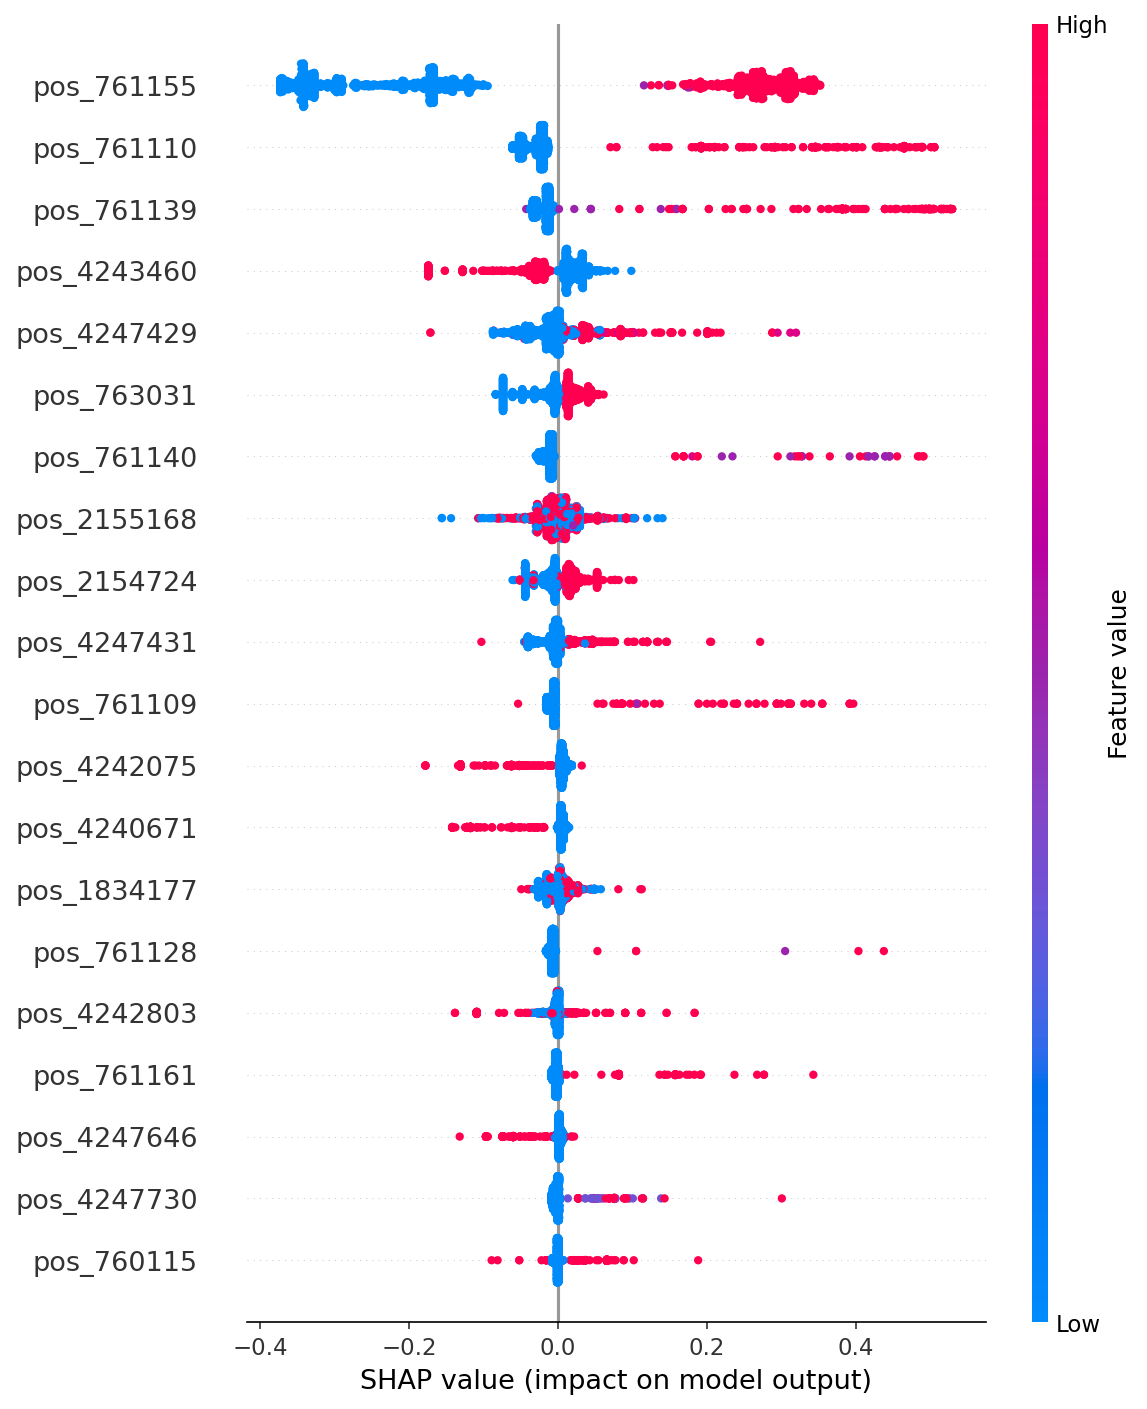
\includegraphics[width=\linewidth]{figures/fig2a_shap_rifampicin.png}
\caption*{(a) Rifampicin}
\end{minipage}
\hfill
\begin{minipage}{0.48\textwidth}
\centering
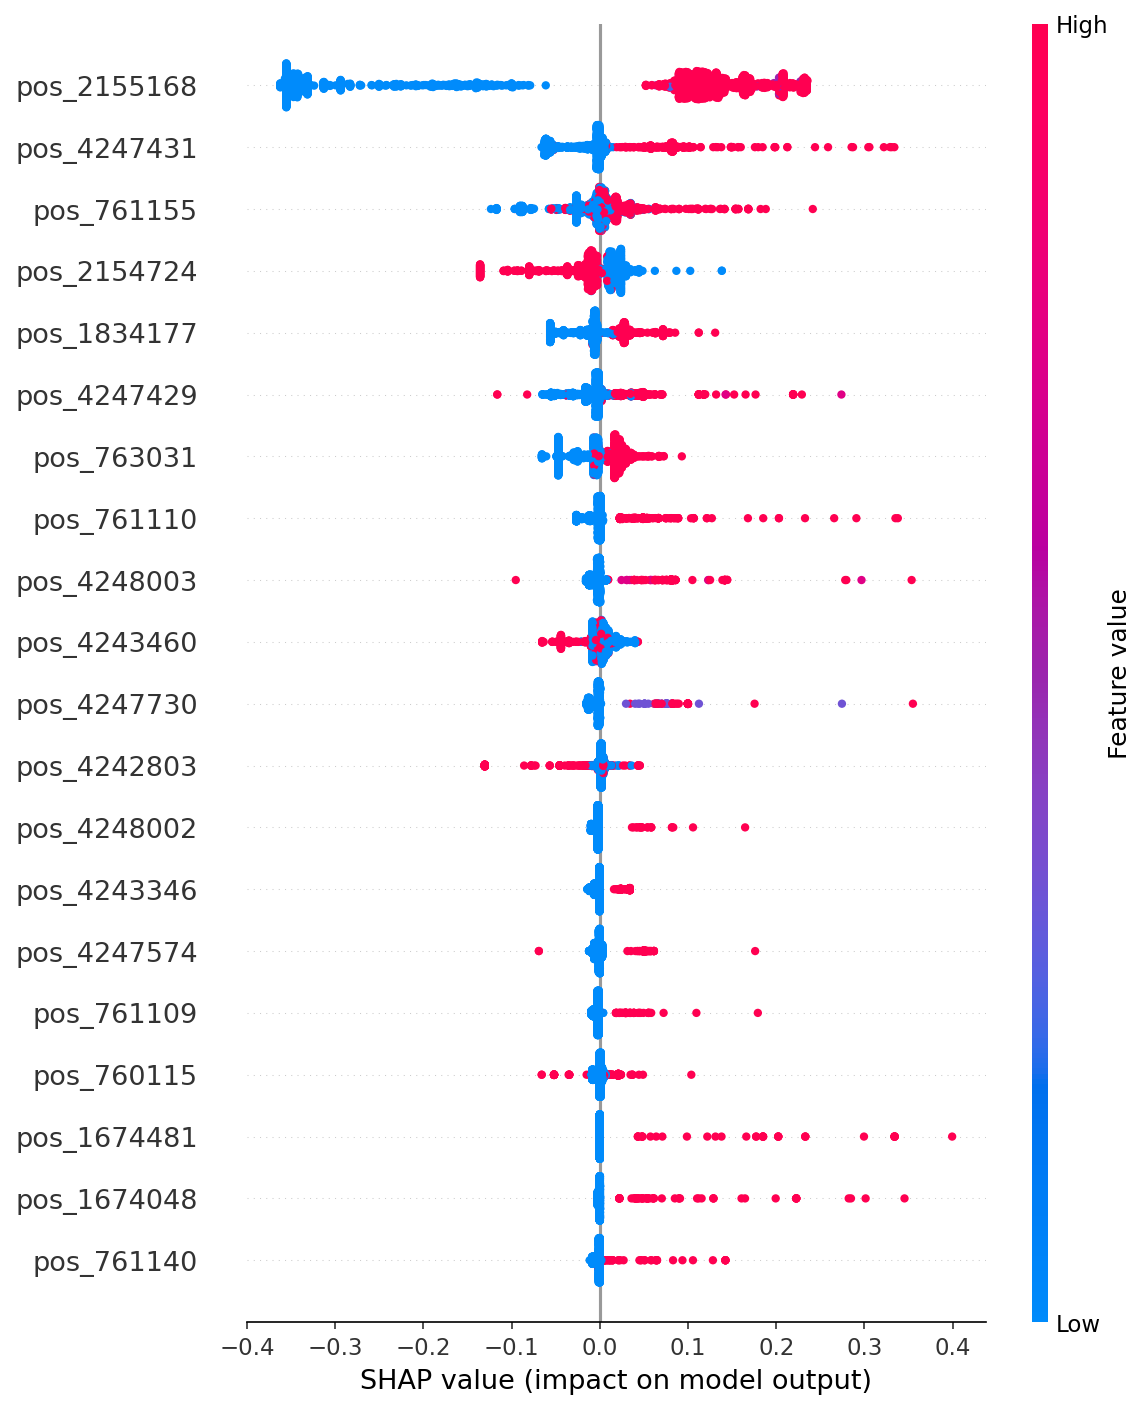
\includegraphics[width=\linewidth]{figures/fig2b_shap_isoniazid.png}
\caption*{(b) Isoniazid}
\end{minipage}

\vspace{6pt}
\begin{minipage}{0.48\textwidth}
\centering
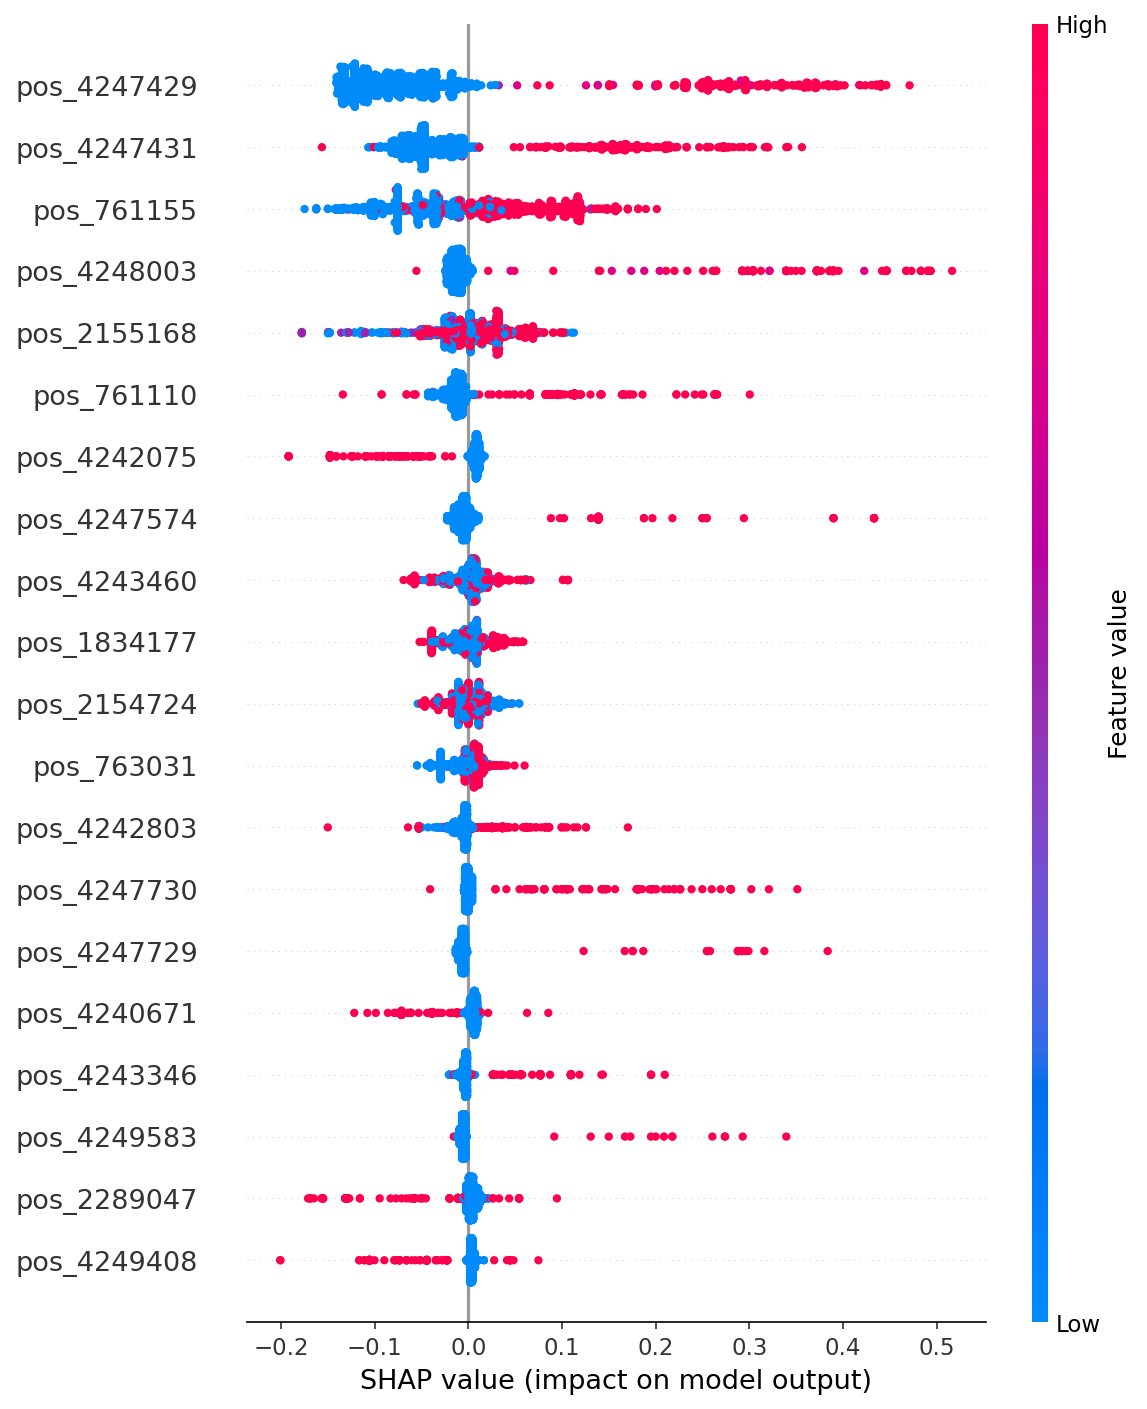
\includegraphics[width=\linewidth]{figures/fig2c_shap_ethambutol.png}
\caption*{(c) Ethambutol}
\end{minipage}
\hfill
\begin{minipage}{0.48\textwidth}
\centering
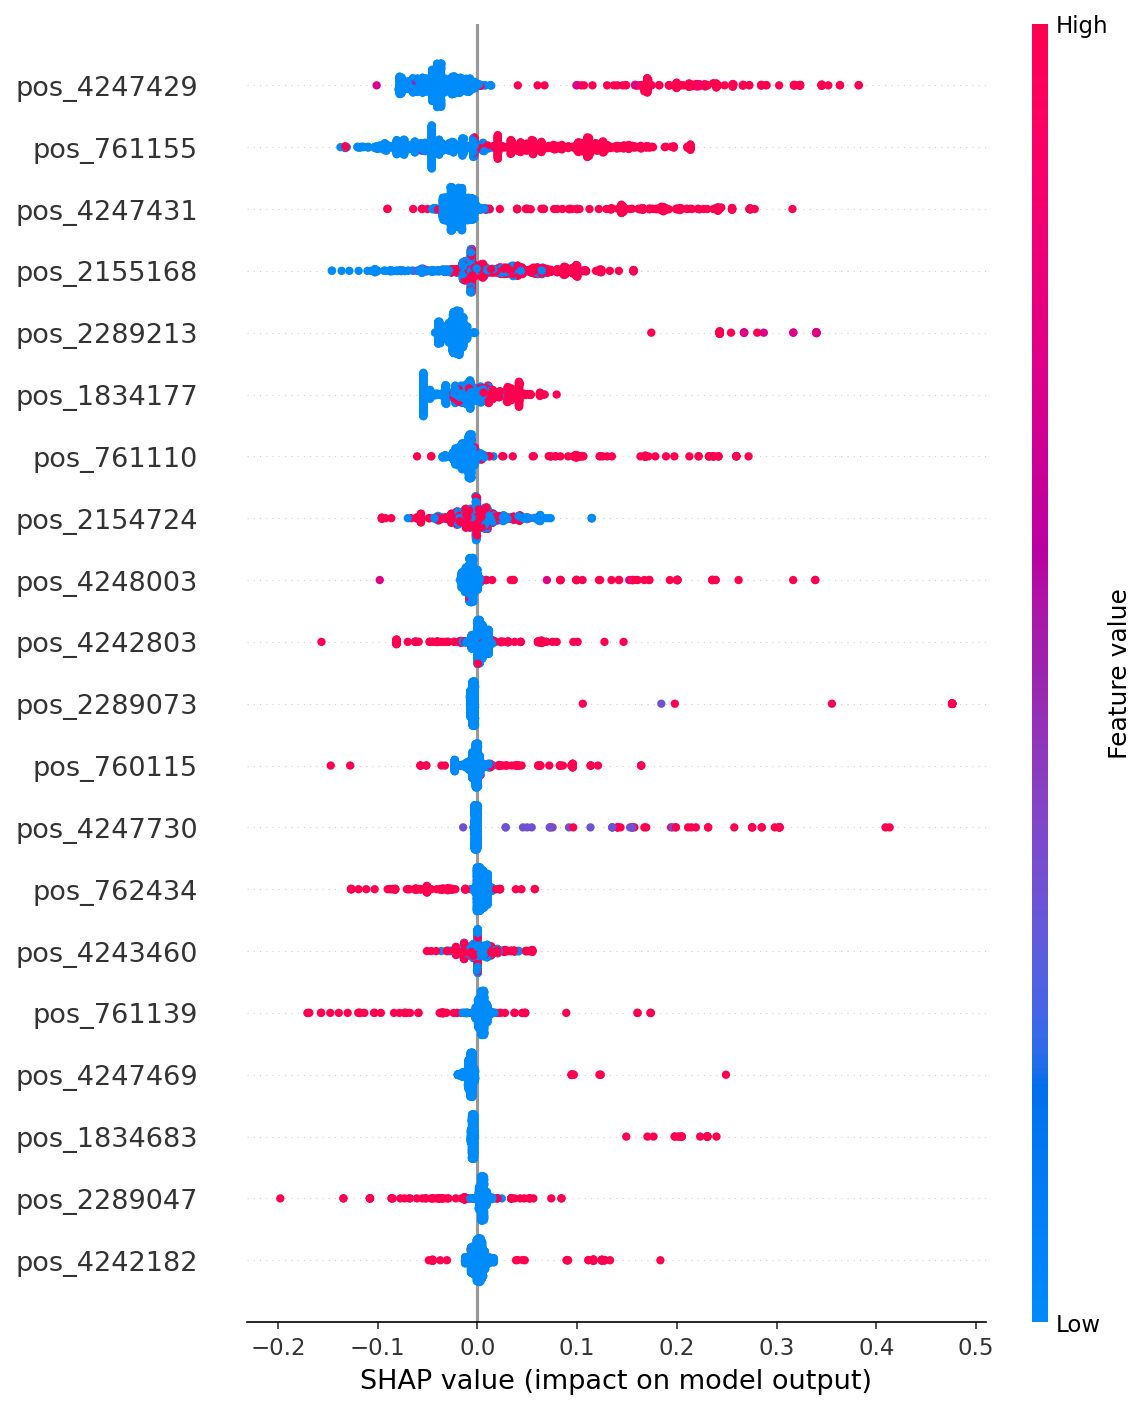
\includegraphics[width=\linewidth]{figures/fig2d_shap_pyrazinamide.png}
\caption*{(d) Pyrazinamide}
\end{minipage}
\caption{SHAP summary (beeswarm) plots for the top-50-feature Random Forest model, one panel per drug. Each point is one isolate; horizontal position is the SHAP value (contribution to predicted resistance log-odds), color encodes the encoded nucleotide value, and features are ranked top-to-bottom by mean absolute SHAP value.}
\label{fig:shap_summary}
\end{figure}

\begin{figure}[h]
\centering
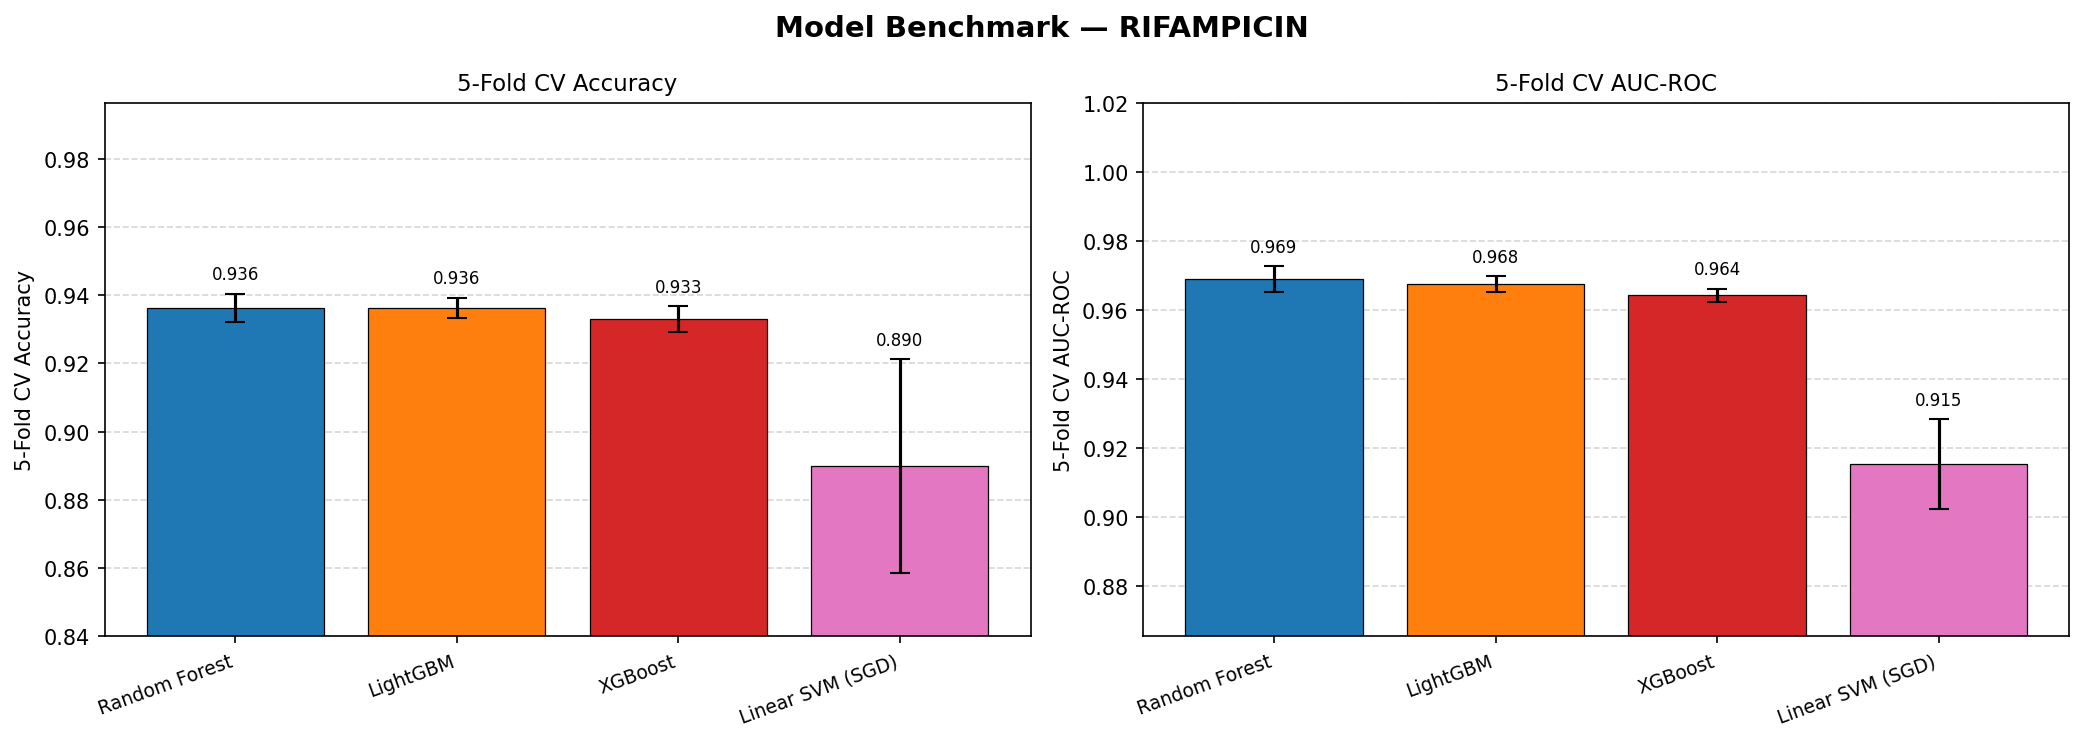
\includegraphics[width=0.85\linewidth]{figures/fig3a_benchmark_rifampicin.png}
\vspace{4pt}
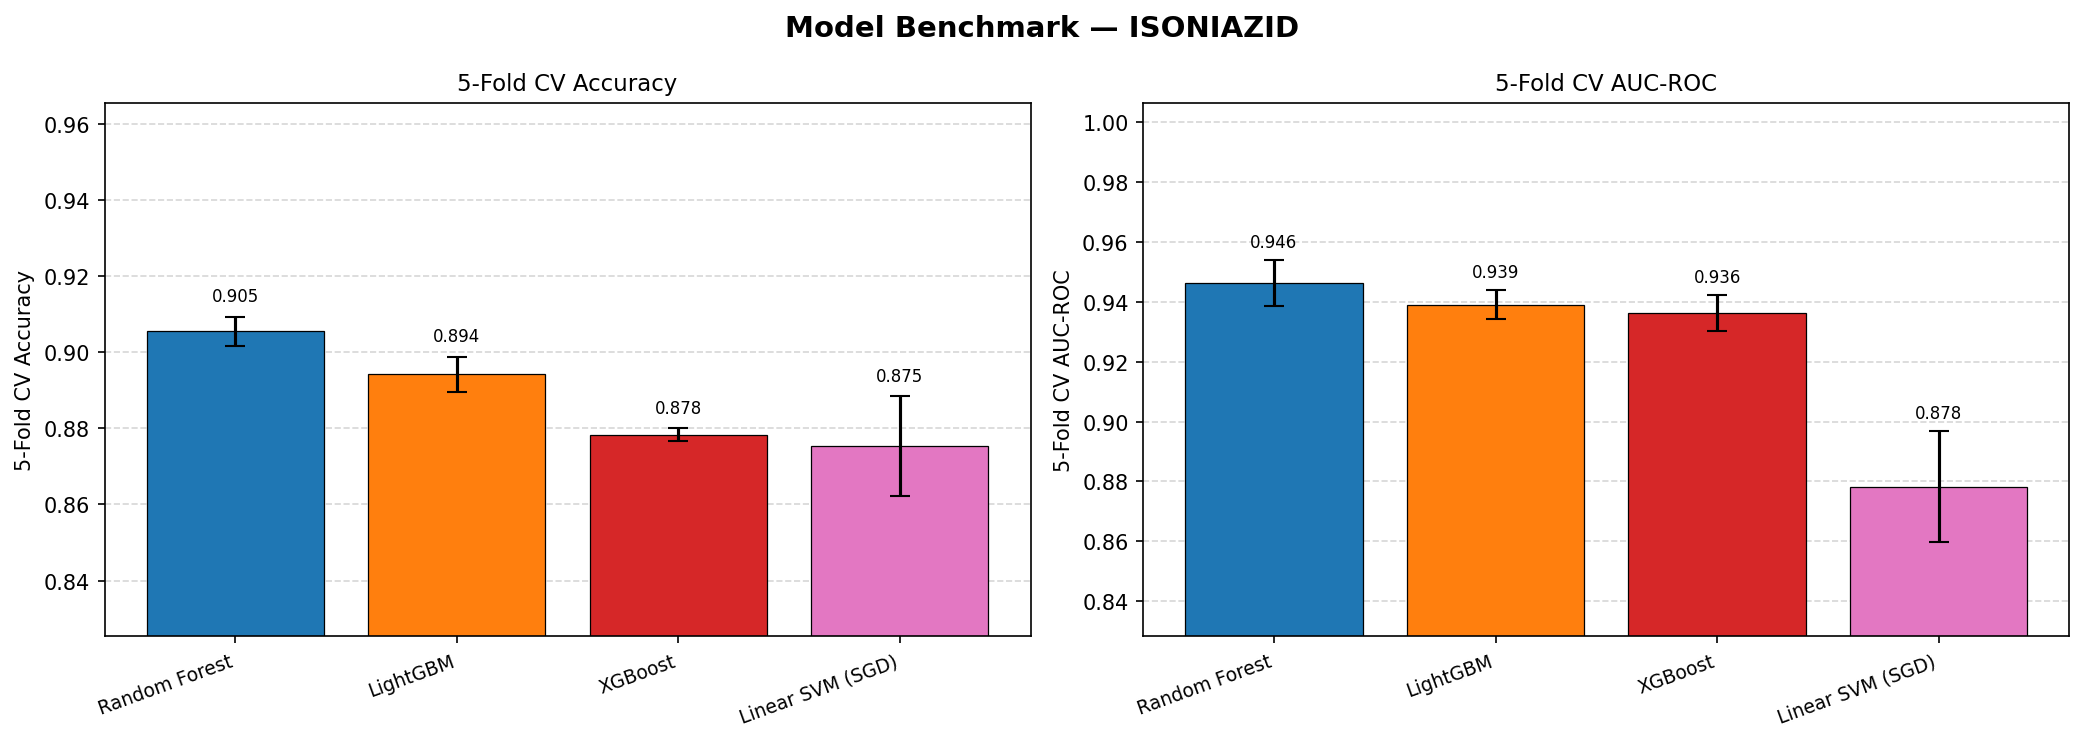
\includegraphics[width=0.85\linewidth]{figures/fig3b_benchmark_isoniazid.png}
\caption{Seven-model CV AUC-ROC comparison for rifampicin (top) and isoniazid (bottom); ethambutol and pyrazinamide follow the same ranking pattern (Random Forest best, linear SVM weakest) per Table~\ref{tab:modelcomparison}.}
\label{fig:benchmark}
\end{figure}

\subsection*{Cross-drug attribution and co-resistance signal}

Because the four drug labels are correlated at the population level (e.g. multidrug-resistant isolates are jointly resistant to rifampicin and isoniazid far more often than expected under independence), we examined whether SHAP attribution for a shared genomic feature shifts between isolates resistant to only one drug versus isolates co-resistant to both. For the rifampicin--isoniazid pair, the dominant rifampicin feature (\emph{rpoB} S450L, pos\_761155) retains a large mean $|\mathrm{SHAP}|$ in the rifampicin model regardless of isoniazid co-resistance status, while several secondary features -- notably the dominant isoniazid feature \emph{katG} S315T (pos\_2155168) -- show a pronounced attribution shift between the single-drug-resistant and co-resistant groups (Table~\ref{tab:crossdrug}). This pattern is consistent with the two mutations reflecting largely independent, drug-specific resistance mechanisms whose co-occurrence in an isolate reflects epidemiological linkage (sequential or concurrent acquisition of MDR-conferring mutations) rather than a shared causal pathway.

\begin{table}[h]
\centering
\caption{Illustrative cross-drug SHAP attribution shift for the rifampicin--isoniazid (RIF--INH) pair: mean $|\mathrm{SHAP}|$ for a shared feature position when isolates are resistant to only one of the two drugs versus co-resistant to both, ranked by the top five positions with the largest attribution shift (max\_abs\_delta).}
\label{tab:crossdrug}
\small
\begin{tabular}{llrrrr}
\toprule
Position & Gene & RIF-only & INH-only & RIF, co-resist. & INH, co-resist. \\
\midrule
pos\_2155168 & katG & 0.026 & 0.239 & 0.011 & 0.122 \\
pos\_761139  & rpoB & 0.120 & 0.002 & 0.040 & 0.002 \\
pos\_761155  & rpoB & 0.289 & 0.023 & 0.271 & 0.018 \\
pos\_761110  & rpoB & 0.052 & 0.011 & 0.065 & 0.008 \\
pos\_2154724 & katG & 0.010 & 0.022 & 0.006 & 0.009 \\
\bottomrule
\end{tabular}

\vspace{4pt}
\footnotesize
The full drug pair yields 41 shared-position rows; the five with the largest attribution shift are shown. pos\_761155 (rpoB S450L) and pos\_2155168 (katG S315T) are the two dominant, independently validated resistance-determining mutations for rifampicin and isoniazid respectively; their recurrence as top-attribution features in each other's models is consistent with population-level co-occurrence of RIF and INH resistance (i.e. MDR-TB) rather than a direct causal cross-drug mechanism.
\end{table}


\subsection*{Multi-label prediction}

Extending Random Forest to jointly predict all four drug labels achieved a macro-averaged AUC-ROC of 0.919 and a Hamming loss of 0.136 (Table~\ref{tab:multilabel}), both consistent with the per-drug AUC-ROC values above. However, subset accuracy -- the fraction of isolates for which all four labels are predicted correctly simultaneously -- was substantially lower at 0.591, reflecting that a single per-drug misclassification anywhere in the four-drug profile counts as a failure under this stricter metric. Random Forest again outperformed LightGBM, XGBoost, and linear SVM on every multi-label metric.

\begin{table}[h]
\centering
\caption{Multi-label (all four RIPE drugs predicted jointly via \texttt{MultiOutputClassifier}) benchmark on the 5{,}180 isolates labelled for all four drugs; plain $K$-fold CV (stratified CV is not defined for multi-label targets).}
\label{tab:multilabel}
\begin{tabular}{lrrr}
\toprule
Model & Hamming Loss $\downarrow$ & Subset Acc. $\uparrow$ & Macro AUC-ROC $\uparrow$ \\
\midrule
Random Forest    & 0.1361 & 0.5907 & 0.9194 \\
LightGBM         & 0.1407 & 0.5753 & 0.9182 \\
XGBoost          & 0.1614 & 0.5106 & 0.9142 \\
Linear SVM (SGD) & 0.1783 & 0.5010 & 0.8282 \\
\bottomrule
\end{tabular}

\vspace{4pt}
\footnotesize
Subset accuracy requires an exact match across all four drug labels simultaneously, a substantially stricter criterion than the per-drug AUC-ROC values in Tables~\ref{tab:perdrug}--\ref{tab:modelcomparison}.
\end{table}


\subsection*{Case study: an MDR-TB isolate}

To illustrate isolate-level interpretability, we applied the trained per-drug models and their SHAP explainers to a held-out demonstration isolate, ERR040120 (Table~\ref{tab:casestudy}). The isolate was predicted resistant to all four drugs, with near-certain probability for rifampicin and isoniazid (both $P=1.000$) driven overwhelmingly by \emph{rpoB} S450L and \emph{katG} S315T respectively, and lower-confidence resistance predictions for ethambutol ($P=0.733$) and pyrazinamide ($P=0.851$) for which no single feature dominates the attribution to the same degree. This isolate and its precomputed explanations are also used as the default "demo mode" input for the public dashboard described below.

\begin{table}[h]
\centering
\caption{Case study: predicted resistance profile for demo isolate ERR040120 (a multidrug-resistant isolate), with its single top-ranked SHAP feature per drug.}
\label{tab:casestudy}
\begin{tabular}{lrll}
\toprule
Drug & $P$(Resistant) & Prediction & Top SHAP feature (gene, SHAP value) \\
\midrule
Rifampicin   & 1.0000 & Resistant & pos\_761155 (rpoB, $+0.2805$) \\
Isoniazid    & 1.0000 & Resistant & pos\_2155168 (katG, $+0.1787$) \\
Ethambutol   & 0.7334 & Resistant & pos\_4247730 (embB, $+0.1480$) \\
Pyrazinamide & 0.8508 & Resistant & pos\_4247730 (embB, $+0.2233$) \\
\bottomrule
\end{tabular}

\vspace{4pt}
\footnotesize
pos\_761155 (rpoB) and pos\_2155168 (katG) correspond to the well-characterized rpoB~S450L and katG~S315T resistance mutations.
\end{table}


\subsection*{Public dashboard}

To make these per-isolate explanations accessible without requiring local computation, we released an interactive Streamlit dashboard, deployed as a public Hugging Face Space. The dashboard supports a demo mode, which loads the precomputed ERR040120 predictions above with no computation required, and a live mode, in which a user-supplied filtered VCF is encoded against the 2{,}693 AMR-gene feature positions, scored using the corresponding per-drug Random Forest model (downloaded from Hugging Face Hub), and explained in real time via \texttt{TreeExplainer}. The dashboard displays a four-drug resistance-profile summary, per-drug SHAP bar charts of the top 20 contributing features, and an expandable table of the underlying mutations, and allows the resulting explanation to be downloaded as JSON.


\section*{Methods}

\subsection*{Data source and reference}

Raw paired-end FASTQ files for 9{,}798 \emph{M. tuberculosis} isolates (after quality-control filtering, described below) were downloaded from the European Nucleotide Archive (ENA) and the NCBI Sequence Read Archive (SRA). All source data are publicly available and de-identified; no patient-identifiable information is included. Phenotypic drug-susceptibility labels were compiled into a master resistance table covering 23{,}051 isolates and 23 drugs in total, of which the four first-line drugs -- rifampicin, isoniazid, ethambutol, and pyrazinamide -- were modelled in this study. Reads were aligned to the H37Rv reference genome (RefSeq NC\_000962.3) \cite{cole1998deciphering}, and gene coordinates were taken from the corresponding GFF annotation (GCF\_000195955.2), restricted to nine genes with established resistance associations: \emph{rpoB} (rifampicin); \emph{katG}, \emph{inhA}, \emph{fabG1} (isoniazid); \emph{embB}, \emph{embA}, \emph{embC} (ethambutol); \emph{pncA}, \emph{rpsA} (pyrazinamide).

\subsection*{Sequence processing pipeline}

The complete framework, from raw sequencing reads through to model interpretation and deployment, is summarized in Fig.~\ref{fig:pipeline}. All processing was performed on the Digital Research Alliance of Canada HPC cluster, orchestrated as per-sample SLURM array jobs with resume protection (skipping samples whose output VCF already existed) and cleanup of intermediate FASTQ/BAM files to conserve scratch storage. The pipeline consisted of the following steps, in order:

\begin{enumerate}
\item \textbf{Download} -- FASTQ retrieval from ENA/SRA via SRA-tools.
\item \textbf{Accession mapping} -- BioSample-to-run accession mapping to resolve one or more sequencing runs per isolate.
\item \textbf{Quality control} -- adapter trimming and quality filtering with fastp \cite{chen2018fastp}.
\item \textbf{Alignment} -- read mapping to H37Rv with BWA-MEM \cite{li2013bwamem}, followed by sorting with SAMtools.
\item \textbf{Variant calling} -- \texttt{bcftools mpileup | bcftools call -mv}, followed by quality filtering (QUAL~$\geq 20$, MQ~$\geq 30$) \cite{danecek2021twelve}.
\end{enumerate}

Software versions and key parameters are summarized in Table~\ref{tab:tools}.

\begin{table}[h]
\centering
\caption{Processing pipeline tool versions and parameters.}
\label{tab:tools}
\begin{tabular}{llll}
\toprule
Step & Tool & Version & Parameters \\
\midrule
Quality control  & fastp          & 1.0.1 & default \\
Alignment        & BWA-MEM        & 0.7.18 & default \\
Variant calling   & bcftools call  & 1.22 & default \\
VCF filtering     & bcftools filter & 1.22 & QUAL~$\geq20$, MQ~$\geq30$ \\
Reference genome  & H37Rv          & NC\_000962.3 & -- \\
\bottomrule
\end{tabular}
\end{table}

\subsection*{Feature matrix construction}

Per-sample filtered VCFs were merged into a single long-format table of 705{,}226 unique variant positions genome-wide. A quality-control pass computed the per-sample variant-count distribution and flagged three isolates (ERR1034652, ERR1035353, ERR1213920) with more than 10{,}000 variants each, well outside the bulk of the distribution and consistent with contamination or platform-specific artefacts; these were excluded from the final dataset. The remaining variants were filtered to (i) single-nucleotide variants only (indels excluded), and (ii) positions intersecting the nine AMR genes listed above. Each retained position was encoded as a single integer column per isolate: 0 for the reference (H37Rv) allele, and 1/2/3/4 for A/T/C/G, respectively; a position absent from an isolate's VCF was assumed to match the reference and encoded as 0. Isolate-level phenotype labels (resistant/susceptible) were joined per drug from the master resistance table. The resulting feature matrix comprises 9{,}798 isolates by 2{,}693 features, with per-drug label availability summarized in Table~\ref{tab:dataset}.

\subsection*{Model training and benchmarking}

For each of the four drugs independently, we trained and benchmarked seven classifiers on an 80/20 stratified train/test split, with 5-fold stratified cross-validation (CV) on the training partition: Random Forest \cite{breiman2001random} (300 trees, \texttt{class\_weight="balanced"}), LightGBM \cite{ke2017lightgbm}, XGBoost \cite{chen2016xgboost}, a linear support vector machine trained via stochastic gradient descent (SGD), and three regularized logistic regression variants (L1/Lasso, ElasticNet, L2/Ridge). Performance was assessed via test-set accuracy and AUC-ROC, and 5-fold CV accuracy and AUC-ROC (mean $\pm$ standard deviation across folds).

To assess joint, multi-drug prediction, we additionally trained a multi-label extension using scikit-learn's \texttt{MultiOutputClassifier} wrapper (Random Forest, LightGBM, XGBoost, and linear SVM base estimators) on the 5{,}180 isolates with phenotype labels available for all four drugs simultaneously. Because stratified cross-validation is not defined for multi-label targets, plain $K$-fold CV was used. Performance was assessed via per-drug and macro-averaged AUC-ROC, Hamming loss (fraction of individual drug labels mispredicted), and subset accuracy (fraction of isolates for which all four drug labels are predicted correctly simultaneously).

\subsection*{SHAP interpretability analysis}

For each drug, the Random Forest model (identified as the best-performing algorithm across all four drugs; see Results) was retrained restricted to its top-50 features by impurity-based importance, and interpreted using \texttt{shap.TreeExplainer} with a 100-sample interventional background dataset \cite{lundberg2017unified}. This produces, for every isolate and every retained feature, a signed SHAP value indicating that feature's contribution to the predicted log-odds of resistance, which we summarize as beeswarm/summary plots per drug (Figure~\ref{fig:shap_summary}) and validate qualitatively against known resistance-determining mutations.

To examine whether feature attributions differ under co-resistance, we performed a cross-drug attribution analysis for all six pairwise combinations of the four drugs. For each drug pair, isolates were partitioned into four resistance-profile groups (resistant to drug A only, drug B only, both -- co-resistant --, or neither), and for each feature shared between the two drugs' top-feature sets we computed the group-wise mean absolute SHAP value and a "delta" metric quantifying the shift in attribution between the single-drug-resistant and co-resistant groups.

\subsection*{Software and computing environment}

Sequence processing used a dedicated conda environment (\texttt{tb-wgs-pipeline}; bioconda/conda-forge channels) containing fastp, BWA, SAMtools, bcftools, and SRA-tools. Downstream feature engineering, modelling, and interpretation used Python with pandas, NumPy, scikit-learn, LightGBM, XGBoost, SHAP, and matplotlib. All HPC jobs were scheduled via SLURM on the Digital Research Alliance of Canada cluster.


\section*{Discussion}

\subsection*{Model selection and the genetic architecture of each drug}

The consistent ranking of Random Forest above gradient-boosted trees, linear SVM, and regularized logistic regression across all four drugs and both the per-drug and multi-label formulations suggests that, on this feature representation, the bagging-based ensemble is more robust than boosting or linear alternatives to the high dimensionality (2{,}693 features), the correlation structure among nearby SNP positions, and the class imbalance of the dataset. The margins are narrow, however -- LightGBM trails Random Forest by 0.0015--0.0132 CV AUC-ROC depending on the drug (Table~\ref{tab:modelcomparison}) -- and with a single train/test split per benchmarking run we cannot claim these differences are statistically meaningful. The honest reading is that the tree ensembles are indistinguishable on this data and the linear models are worse.

The performance ordering across drugs is more informative than the ordering across models. Rifampicin and isoniazid resistance are each driven predominantly by a small number of high-penetrance mutations in \emph{rpoB} and \emph{katG} respectively \cite{who2023catalogue,walker2015whole}, which a classifier can exploit almost as a near-deterministic rule. Pyrazinamide is the opposite case: resistance is conferred by loss of \emph{pncA} function, and the substitutions that cause it are distributed across the entire length of the gene without hotspots -- more than 300 resistance-conferring substitutions have been characterized, many acting by reducing PncA protein abundance rather than by altering a catalytic residue \cite{yadon2017pnca}. A feature set of individual nucleotide positions is structurally ill-suited to that architecture: each causal variant is individually rare, so no single column carries much signal. This is a limitation of the representation, not of the classifier, and it bounds what any position-encoded model can achieve for this drug.

\subsection*{Performance in context: this pipeline is not state of the art}

The per-drug AUC-ROC values reported here (0.883--0.976) are at or below what established tools already achieve. TB-Profiler \cite{phelan2019tbprofiler} and the machine-learning-based GenTB \cite{groschel2021gentb} are both mature, widely deployed predictors covering 13 drugs; GenTB's own benchmark against 20{,}408 phenotyped isolates reports mean sensitivities of 77.6\% (GenTB random forest), 75.4\% (GenTB wide-and-deep network), 74.4\% (TB-Profiler) and 71.9\% (Mykrobe) across nine shared drugs, at specificities above 96\% \cite{groschel2021gentb}. For the multi-label problem specifically, DeepAMR \cite{yang2019deepamr} -- a multi-task denoising autoencoder built for co-occurrent resistance, the same problem our \texttt{MultiOutputClassifier} extension addresses -- reports AUCs of 0.944--0.987 on the first-line drugs, comfortably above our macro AUC-ROC of 0.919 and against a far more demanding target.

We therefore do not claim competitive accuracy, and this manuscript should not be read as proposing a replacement for those tools. Two caveats cut in both directions. First, cross-study comparison of these numbers is not sound: cohorts, label provenance, critical concentrations, train/test partitioning and drug coverage all differ, and benchmarking work has shown that reported performance for TB resistance prediction is strongly sensitive to which database and which isolate set is used \cite{ngo2019benchmarking}. Our own numbers are no more comparable to DeepAMR's than DeepAMR's are to TB-Profiler's. Second, that non-comparability is itself an indictment of the field rather than a defence of our results: without a shared, versioned benchmark it is not possible to say whether any of these methods is actually better than another. The contribution we can defend is the openly released feature matrix, code, models and per-isolate explanation layer -- infrastructure that makes such a comparison easier -- not the accuracy of the classifiers built on top of it.

\subsection*{Label quality bounds what can be learned}

A model can be no better than its labels, and ours are heterogeneous: phenotypes were aggregated across many source studies with unrecorded testing methods and critical concentrations. This matters most for pyrazinamide. Phenotypic pyrazinamide susceptibility testing in the Bactec MGIT 960 system is well documented to produce false-resistant results, driven by inoculum density and medium acidification, with reported false-resistance rates in the tens of percent and substantial improvement when inoculum is reduced \cite{mok2021pza,mustazzolu2019revisiting}. Some fraction of the pyrazinamide labels used here is therefore likely to be wrong, and in a specific direction: susceptible isolates mislabelled as resistant. Our weaker pyrazinamide performance consequently confounds three distinct effects -- a genuinely harder genetic architecture, a representation unsuited to it, and noisy ground truth -- and the present design cannot separate them. Any future evaluation of this pipeline on pyrazinamide should use a cohort with documented, quality-controlled DST, or quantitative MIC phenotypes of the kind assembled by the CRyPTIC compendium \cite{cryptic2022compendium}, rather than pooled binary calls.

\subsection*{Limitations of the SHAP analysis itself}

The interpretability layer, which is the paper's main claim to novelty, rests on assumptions this dataset violates. Shapley-value attributions are defined by averaging a feature's marginal contribution over subsets of the remaining features, and the standard estimators assume those features can be varied independently. Genomic features are the textbook case where that fails: linkage disequilibrium, the clonal population structure of the \emph{M. tuberculosis} complex, and the co-resistance correlation we ourselves report all create strong dependence between columns. Under dependent features, marginal (interventional) Shapley estimators evaluate the model off the data manifold and can distribute credit in ways that do not reflect the conditional structure of the data \cite{aas2021explaining}. Our use of a 100-sample interventional background in \texttt{TreeExplainer} is precisely this setting, and the background is small. More fundamentally, Shapley values are a mathematical allocation, not a causal or human-facing explanation; the properties that make them attractive do not by themselves license the inferences users tend to draw from them, and recovering them for causal purposes requires assumptions the method does not supply \cite{kumar2020problems}. Two consequences follow for this work. Attribution split between two tightly linked positions should not be interpreted as evidence about which is functional; and our restriction of the SHAP analysis to the top 50 features by impurity importance imposes a prior selection step whose effect on the resulting attributions we did not quantify.

The recovery of \emph{rpoB} S450L, \emph{katG} S315T and \emph{embB} M306 should be read in that light. It is a necessary sanity check, and it is reassuring that the pipeline is not learning something spurious -- but it is weak validation. These are the most prevalent resistance mutations globally \cite{who2023catalogue}, so any competent model trained on this data would surface them, and recovering known biology demonstrates the absence of an obvious failure rather than the presence of new insight.

\subsection*{Cross-drug attribution and population structure}

The cross-drug analysis shows that resistance-associated features for one drug (e.g. \emph{katG} S315T) retain measurable attribution in a different drug's model, with no known mechanistic link. The most parsimonious explanation is population-level linkage between resistance mutations in MDR/XDR lineages rather than a causal cross-drug effect. This is a recognized hazard for machine learning on this organism specifically: the \emph{M. tuberculosis} complex has a highly clonal population structure, with negligible horizontal gene transfer and low recombination, so isolates are not statistically independent and models can learn lineage markers that travel with resistance rather than the determinants themselves \cite{billows2023feature}. Our pooled, lineage-agnostic design does nothing to guard against this. We therefore present the cross-drug attribution shifts as a measurement of correlation structure in the training data, not as a biological finding; on the evidence available they are as consistent with confounding as with anything else, and we would discourage readers from reading them as novel resistance biology. Methods for the problem already exist -- stratification, lineage-aware feature selection, and feature-weighted random forests have all been evaluated for exactly this task \cite{billows2023feature} -- and applying one is the single most important next step for this pipeline.

\subsection*{Class imbalance and the value of a susceptible call}

Class imbalance is substantial for two of the four drugs (isoniazid 86.0\% resistant; rifampicin 74.2\% resistant), reflecting a cohort assembled from resistance-focused studies rather than a representative clinical population. While \texttt{class\_weight="balanced"} mitigates its effect during training, headline accuracy and AUC-ROC on an imbalanced test set obscure where the model actually fails: isoniazid susceptible-class precision is 0.61 against 0.98 for the resistant class (Table~\ref{tab:perdrug}). In clinical terms the more consequential error -- calling a resistant isolate susceptible, and thereby endorsing an ineffective regimen -- is the one the imbalance makes hardest to characterize reliably, because susceptible isolates are scarce in the test split. A prospective, consecutively sampled cohort would be needed to estimate that error rate honestly.

\subsection*{Relation to curated catalogues}

Relative to rule-based catalogues such as the WHO catalogue of mutations, now in its second edition and covering more than 30{,}000 variants derived from over 52{,}000 isolates \cite{who2023catalogue}, this pipeline trades curated certainty for (i) native support for four drugs from a single unified pipeline, (ii) a continuous, per-isolate quantitative explanation rather than a binary present/absent mutation flag, and (iii) the ability to surface signal the catalogue does not encode without waiting for a re-curation cycle. The comparison should not be read as a contest. Curated catalogues carry expert adjudication and a documented evidence grade per variant that a learned model has no equivalent of, and independent evaluation on regional cohorts is how their real diagnostic performance has been established \cite{garciamarin2024role}. A catalogue and a model are complementary: the catalogue is the reference standard against which an attribution should be checked, and unexplained attribution is a lead to investigate rather than a finding in itself.

\subsection*{Limitations}

Beyond the issues above, several constraints bound this work. The feature set is restricted to single-nucleotide variants within nine known AMR genes, so indels and structural variants -- which contribute substantially to loss of \emph{pncA} function \cite{yadon2017pnca} -- are excluded entirely, and restricting to known genes forecloses discovery of determinants outside them. Evaluation used a single train/test split per benchmarking run rather than repeated splits or a held-out external cohort, so the reported differences between models carry no confidence intervals and generalization to under-represented regions and lineages is untested. Only four of the 23 drugs present in the underlying phenotype table were modelled. The reference-matching encoding treats any position absent from a sample's VCF as wild type, which conflates true reference calls with positions of low coverage and will systematically underestimate variant burden in poorly sequenced isolates. Finally, the demonstration isolate used for the case study is a single MDR sample and illustrates the output format rather than validating it.

\subsection*{Future directions}

These limitations suggest a clear order of priority. Lineage-aware modelling comes first, since it determines whether the cross-drug findings reported here are biological or artefactual, and established methods for this dataset type are available to adopt rather than invent \cite{billows2023feature}. Second, the interpretability layer should be re-derived with estimators that respect feature dependence \cite{aas2021explaining}, and the effect of the top-50 pre-selection quantified, before any attribution is offered as evidence about a specific locus. Third, evaluation should move to an external cohort with documented phenotyping -- the CRyPTIC compendium \cite{cryptic2022compendium} offers quantitative MICs and would allow the pyrazinamide label-noise question to be separated from the representation question -- and should report against the same isolates used by existing tools so that a genuine comparison with TB-Profiler, GenTB and DeepAMR becomes possible \cite{phelan2019tbprofiler,groschel2021gentb,yang2019deepamr,ngo2019benchmarking}. Fourth, the representation should move beyond individual nucleotide positions toward variant- or protein-level features that can aggregate rare loss-of-function events, which is where the pyrazinamide gains are most likely to come from. Extension to second-line drugs and richer feature types follows from these.

Taken together, this work demonstrates that an interpretable, multi-drug pipeline can be assembled end to end from public sequencing data and open-source tooling, and released in full. Its value lies in that reproducibility and in the per-isolate explanation layer, not in predictive performance, which trails established tools. We offer FORUM-TB as a transparent baseline and a shared resource against which more sophisticated, lineage-aware and clinically validated interpretable models can be developed and -- given a common benchmark -- fairly compared.


\section*{Data and Code Availability}

The processing pipeline, modelling code, and this manuscript's source are available at \url{https://github.com/TheMicrobialist/SHAP-mTB-AMR} (v0.2.0). The interactive dashboard is deployed as a public Hugging Face Space. All data are derived from publicly available, de-identified ENA/SRA sequencing runs. The dataset and code are released under a CC BY-NC 4.0 license.

\section*{Acknowledgments}

Sequence processing was performed on the Digital Research Alliance of Canada HPC infrastructure.


\bibliographystyle{IEEEtran}
\bibliography{references}

\end{document}
